\documentclass{article}

\usepackage{pandekten}
\usepackage{dashrule}

\makeatletter
\newcommand*{\shifttext}[1]{%
  \settowidth{\@tempdima}{#1}%
  \hspace{-\@tempdima}#1%
}
\newcommand{\plabel}[1]{%
\shifttext{\textbf{#1}\quad}%
}
\newcommand{\prule}{%
\begin{center}%
\hdashrule[0.5ex]{.99\linewidth}{1pt}{1pt 2.5pt}%
\end{center}%
}

\makeatother

\newcommand{\minusbaseline}{\abovedisplayskip=0pt\abovedisplayshortskip=0pt~\vspace*{-\baselineskip}}%

\setlength{\parindent}{0pt}

\title{Assignment 6}
\author{Ze Chen}

\begin{document}

\maketitle

\plabel{1 (a)}%
\begingroup\minusbaseline
\begin{align*}
    \dot{N}_1 &= -\Gamma_p N_1 + \gamma_{13}N_3 + \gamma_{12}N_2, \\
    \dot{N}_2 &= \gamma_{23}N_3 - \gamma_{12}N_2, \\
    \dot{N}_3 &= \Gamma_p N_1 - \gamma_{13}N_3 - \gamma_{23}N_3.
\end{align*}
\endgroup

\plabel{(b)}%
Majority in state 1.

\plabel{(c)}%
Let $\dot{N}_i = 0$.
We find
\[ N_1 = \frac{\gamma_{13}+\gamma_{23}}{\Gamma_p} N_3,\quad N_2 = \frac{\gamma_{23}}{\gamma_{12}} N_3. \]
Since $N_A = N_1 + N_2 + N_3$, for $N_2 > N_1$ we find
\[ \Gamma_p > \frac{\gamma_{12}(\gamma_{13}+\gamma_{23})}{\gamma_{23}}. \]

\plabel{(d)}%
Since
\[ \frac{N_2}{N_1} = \Gamma_p \cdot \frac{\gamma_{23}}{\gamma_{12}(\gamma_{13}+\gamma_{23})}. \]
we need quick $\gamma_{23}$ and slow $\gamma_{12}$, $\gamma_{13}$.

\plabel{(e)}%
The steady state displays oscillation and spatial dependence.

\prule

\plabel{2 (a)}%
$P = \rho p$, where $\rho = n/V$.

\plabel{(b)}%
\begingroup\minusbaseline
\begin{align*}
    \grad^2 E - \frac{n^2}{c^2} \pdv[2]{E}{t} &= \mu_0 \pdv[2]{}{t}\qty(P^+ + P^-), \\
    \dot{P}^+(x,t) &= (-i\omega_{12} - \gamma_\perp) P^+(x,t) - \frac{i\mathcal{P}_{12}^2}{\hbar} E \cdot D, \\
    \dot{D} &= -\gamma_{\parallel}(D - D_0) + \frac{2i}{\hbar}E\cdot (P^- - P^+),
\end{align*}
\endgroup
where
\[ D_0 = \rho\qty(\frac{\Gamma_p}{\gamma_{\parallel}} - 1). \]
$D_0$ is the steady state when $E=0$ for the inversion equation, without loss of photons in the leaky cavity taken into account.

\plabel{(c)}%
Let
\begin{align*}
    E(x,t) &= \sum_m e_m(t) \varphi_m(x), \\
    P(x,t) &= \sum_m p_m(t) \varphi_m(x).
\end{align*}
From the equation for $\dot{P}$ we find
\[ \dot{p}_m = (-i\gamma_{12} - \gamma_\perp) p_m - \frac{i\mathcal{P}^2_{12}}{\hbar} \sum_{n} d_{mn}(t) e_{n}(t) \]
where
\[ d_{mn}(t) = \int \varphi^*_m \cdot D \cdot \varphi_n \dd{x}. \]
From the equation for $\dot{D}$ we find
\[ \dot{d}_{mn} = -\gamma_\parallel(d_{mn} - D_0 \delta_{mn}) + \frac{2i}{\hbar}\sum_{r,s}\qty(e_r \cdot p^*_s \int \varphi^*_m \varphi_r \varphi_s^* \varphi_n \dd{x} - \text{h.c.}). \]
From the equation for $\dot{E}$ we find
\[ -\ddot{e}_m - \omega^2_m e_m = \frac{c^2\mu_0}{n^2} \ddot{p}_m. \]

\plabel{(d)}%
\begingroup\minusbaseline
\begin{align*}
    \ddot{e}_M + \omega_M^2 e_M &= -\frac{1}{\epsilon_0 n^2} \ddot{p}_M, \\
    \dot{p}_M &= (-i\omega_{12} - \gamma_\perp) p_M - \frac{i\mathcal{P}_{12}^2}{\hbar} d_M e_M, \\
    \dot{d}_M &= -\gamma_{\parallel} (d_M - D_0) + \frac{2i}{\hbar V_M}(e_M p_M^* - e_M^* p_M),
\end{align*}
\endgroup
where
\[ V_M = \qty(\int \dd{x} \abs{\varphi_M(x)}^4)^{-1} \]
represents the inverse of the power of the wave due to the geometry of the cavity.

\plabel{(e)}%
From the equation for $p$ we find
\[ \overline{p} = \frac{i\mathcal{P}_{12}^2 d_M \overline{e}_M/\hbar}{i(\Omega - \omega_{12}) - \gamma_\perp}. \]
From the equation for $d$ we find
\[ d_M = \frac{D_0}{1 + 4 g(\Omega) I_M / I_{\mathrm{SAT}}} \]
where
\[ g(\Omega) = \frac{\gamma_\perp^2 / V_M}{\Delta^2 + \gamma_\perp^2} \]
and
\[ I_{\mathrm{SAT}} = \frac{\hbar^2 \gamma_\perp \gamma_\parallel}{\mathcal{P}^2_{12}}. \]
From the equation for $e$ we find
\[ \frac{1}{2n^2 \epsilon_0} \frac{\Omega}{\Omega - \omega_M} \frac{\mathcal{P}_{12}^2 / \hbar}{\Omega - \omega_{12} + i\gamma_\perp} \frac{D_0}{1+4g(\Omega) I_M / I_{\mathrm{SAT}}} = -1. \]
Let $\omega_M = \nu_M - i\kappa_M$.
Then
\[ \Omega = \frac{\gamma_\perp}{\gamma_\perp + \kappa_M} \nu_M + \frac{\kappa_M}{\gamma_\perp + \kappa_M} \omega_{12}. \]
Finally,
\begin{align*}
    d_{\mathrm{th}} &= \frac{d_0}{1+4g(\Omega) I_M / I_{\mathrm{SAT}}}, \\
    I_M &= \frac{I_{\mathrm{SAT}}}{4g(\Omega)}\qty(\frac{d_0}{d_{\mathrm{th}}} - 1).
\end{align*}

\prule
\plabel{3 (a)}%
For $D_{\mathrm{th}}$ to be lower, we use smaller $\kappa_M$ and $(\Omega-\omega_{12})^2$.
To increase the slope efficiency $\sim V_M I_{\mathrm{SAT}}/\kappa_M$, we may increase $V_M$ and decrease $\kappa_M$.

\plabel{(b)}%
Before threshold, $d_M = D_0$.
After threshold, $d_M = D_{\mathrm{th}}$.
The effect is called gain clamping.
The power will continue to increase if we increase the pumping frequency since $I_M \propto (D_0/D_{\mathrm{th}} - 1)$.

\plabel{(c)}%
\begingroup\minusbaseline
\[ D = \frac{D_0}{1+4g\abs{\varphi_M(x)}^2 I_m/I_{\mathrm{SAT}}}. \]
\endgroup
For a ring cavity, $D$ is constant.
\begin{center}
    \begin{tikzpicture}[scale=0.5]
        \begin{axis}[
            ticks=none,axis x line=bottom,axis y line=left,
            xlabel={$x$},
            ylabel={$D$},
        ]
            \addplot [mark=none,domain=0:pi] {1};
        \end{axis}
    \end{tikzpicture}
\end{center}
For a Fabry-Perot etalon, the plot is given below.
\begin{center}
    \begin{tikzpicture}[scale=0.5]
        \begin{axis}[
            ticks=none,axis x line=bottom,axis y line=left,
            xlabel={$x$},
            ylabel={$D$},
            ymin=0,
            ymax=2.1,
        ]
            \addplot [mark=none,domain=0:pi,samples=200] {2/(1+0.1*sin(deg(x)*3)^2)};
        \end{axis}
    \end{tikzpicture}
\end{center}
The power is not optium and $D$ is smaller in some part than elsewhere.

\plabel{(d)}%
\begingroup\minusbaseline
\begin{align*}
    \omega_m &= \frac{2\pi m c}{Ln}, \\
    \nu_m &= \frac{2\pi m c}{L \abs{n}^2} \Re n, \\
    \kappa_m &= \frac{2\pi m c}{L \abs{n}^2} \Im n, \\
    \varphi_m(x) &= \frac{1}{\sqrt{L}} e^{2\pi i m x/L}.
\end{align*}
\endgroup

\plabel{(e)}%
\begingroup\minusbaseline
\begin{align*}
    g(\omega) &\propto \frac{\gamma^2_\perp}{(\omega - \omega_{12})^2 + \gamma_\perp^2}, \\
    \Omega_M &= \frac{\gamma_\perp}{\gamma_\perp + \kappa_M}\nu_M + \frac{\kappa_M}{\gamma_\perp + \kappa_M} \omega_{12}, \\
    \Re \omega_m &= \frac{2\pi m c}{L\abs{n}^2} \Re n.
\end{align*}
\endgroup

\begin{center}
    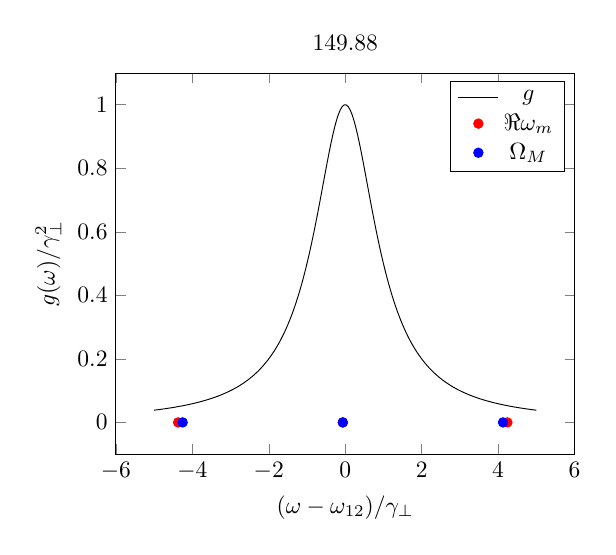
\begin{tikzpicture}[scale=0.85]
        \begin{axis}[
            xlabel={$(\omega-\omega_{12})/\gamma_\perp$},
            ylabel={$g(\omega)/\gamma_\perp^2$},
            title=\SI{149.88}{\micro\meter}
        ]
            \addplot[mark=none,domain=-5:5,samples=200] {1/(x^2+1)};
            \addplot[only marks, draw=red, fill=red] coordinates {
                (-4.3705, 0.)
                (-0.0635073, 0.)
                (4.24349, 0.)
            };
            \addplot[only marks, draw=blue, fill=blue] coordinates {
                (-4.25216, 0.)
                (-0.0617846, 0.)
                (4.12817, 0.)
            };
            \legend{$g$, $\Re \omega_m$, $\Omega_M$}
        \end{axis}
    \end{tikzpicture}
\end{center}

\begin{center}
    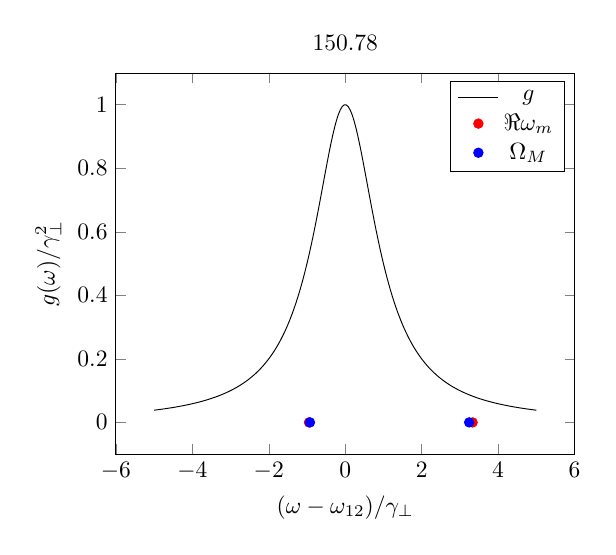
\begin{tikzpicture}[scale=0.85]
        \begin{axis}[
            xlabel={$(\omega-\omega_{12})/\gamma_\perp$},
            ylabel={$g(\omega)/\gamma_\perp^2$},
            title=\SI{150.78}{\micro\meter}
        ]
            \addplot[mark=none,domain=-5:5,samples=200] {1/(x^2+1)};
            \addplot[only marks, draw=red, fill=red] coordinates {
                (-0.947873, 0.)
                (3.33342, 0.)
            };
            \addplot[only marks, draw=blue, fill=blue] coordinates {
                (-0.92217, 0.)
                (3.24286, 0.)
            };
            \legend{$g$, $\Re \omega_m$, $\Omega_M$}
        \end{axis}
    \end{tikzpicture}
\end{center}

\begin{center}
    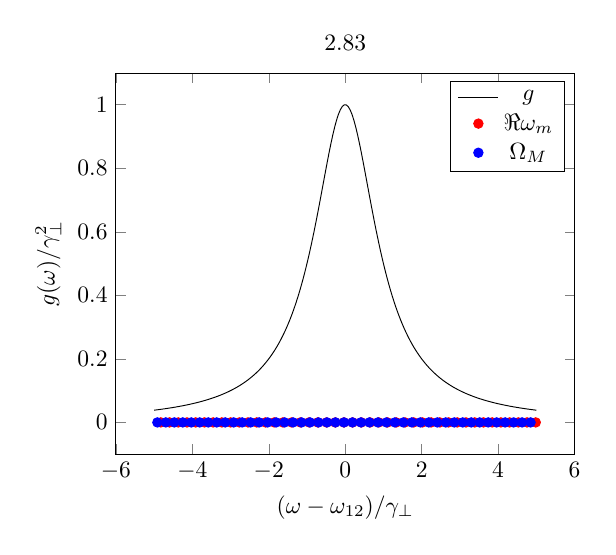
\begin{tikzpicture}[scale=0.85]
        \begin{axis}[
            xlabel={$(\omega-\omega_{12})/\gamma_\perp$},
            ylabel={$g(\omega)/\gamma_\perp^2$},
            title=\SI{2.83}{\milli\meter}
        ]
            \addplot[mark=none,domain=-5:5,samples=200] {1/(x^2+1)};
            \addplot[only marks, draw=red, fill=red] coordinates {
                (-4.82318, 0.)  (-4.59508, 0.)  (-4.36697, 0.)  (-4.13887, 0.)  
(-3.91077, 0.)  (-3.68266, 0.)  (-3.45456, 0.)  (-3.22646, 0.)  
(-2.99835, 0.)  (-2.77025, 0.)  (-2.54215, 0.)  (-2.31404, 0.)  
(-2.08594, 0.)  (-1.85784, 0.)  (-1.62973, 0.)  (-1.40163, 0.)  
(-1.17353, 0.)  (-0.945422, 0.)  (-0.717319, 0.)  (-0.489215, 0.)  
(-0.261112, 0.)  (-0.0330083, 0.)  (0.195095, 0.)  (0.423199, 0.)  
(0.651302, 0.)  (0.879405, 0.)  (1.10751, 0.)  (1.33561, 0.)  
(1.56372, 0.)  (1.79182, 0.)  (2.01992, 0.)  (2.24803, 0.)  (2.47613, 
0.)  (2.70423, 0.)  (2.93234, 0.)  (3.16044, 0.)  (3.38854, 0.)  
(3.61665, 0.)  (3.84475, 0.)  (4.07285, 0.)  (4.30096, 0.)  (4.52906, 
0.)  (4.75716, 0.)  (4.98527, 0.)
            };
            \addplot[only marks, draw=blue, fill=blue] coordinates {
                (-4.91455, 0.)  (-4.69261, 0.)  (-4.47067, 0.)  (-4.24873, 0.)  
(-4.02679, 0.)  (-3.80485, 0.)  (-3.58292, 0.)  (-3.36098, 0.)  
(-3.13905, 0.)  (-2.91712, 0.)  (-2.69519, 0.)  (-2.47326, 0.)  
(-2.25133, 0.)  (-2.0294, 0.)  (-1.80748, 0.)  (-1.58555, 0.)  
(-1.36363, 0.)  (-1.14171, 0.)  (-0.919786, 0.)  (-0.697866, 0.)  
(-0.475947, 0.)  (-0.254029, 0.)  (-0.0321129, 0.)  (0.189802, 0.)  
(0.411716, 0.)  (0.633629, 0.)  (0.855541, 0.)  (1.07745, 0.)  
(1.29936, 0.)  (1.52127, 0.)  (1.74318, 0.)  (1.96508, 0.)  (2.18699, 
0.)  (2.40889, 0.)  (2.63079, 0.)  (2.85269, 0.)  (3.07459, 0.)  
(3.29649, 0.)  (3.51839, 0.)  (3.74028, 0.)  (3.96218, 0.)  (4.18407, 
0.)  (4.40596, 0.)  (4.62786, 0.)  (4.84975, 0.)
            };
            \legend{$g$, $\Re \omega_m$, $\Omega_M$}
        \end{axis}
    \end{tikzpicture}
\end{center}

\SI{149.88}{\micro\meter} and \SI{150.78}{\micro\meter} are candidates since they have few modes close to the center.

% \bibliographystyle{plain}
% \bibliography{main}

\end{document}

